\documentclass[1p]{elsarticle_modified}
%\bibliographystyle{elsarticle-num}

%\usepackage[colorlinks]{hyperref}
%\usepackage{abbrmath_seonhwa} %\Abb, \Ascr, \Acal ,\Abf, \Afrak
\usepackage{amsfonts}
\usepackage{amssymb}
\usepackage{amsmath}
\usepackage{amsthm}
\usepackage{scalefnt}
\usepackage{amsbsy}
\usepackage{kotex}
\usepackage{caption}
\usepackage{subfig}
\usepackage{color}
\usepackage{graphicx}
\usepackage{xcolor} %% white, black, red, green, blue, cyan, magenta, yellow
\usepackage{float}
\usepackage{setspace}
\usepackage{hyperref}

\usepackage{tikz}
\usetikzlibrary{arrows}

\usepackage{multirow}
\usepackage{array} % fixed length table
\usepackage{hhline}

%%%%%%%%%%%%%%%%%%%%%
\makeatletter
\renewcommand*\env@matrix[1][\arraystretch]{%
	\edef\arraystretch{#1}%
	\hskip -\arraycolsep
	\let\@ifnextchar\new@ifnextchar
	\array{*\c@MaxMatrixCols c}}
\makeatother %https://tex.stackexchange.com/questions/14071/how-can-i-increase-the-line-spacing-in-a-matrix
%%%%%%%%%%%%%%%

\usepackage[normalem]{ulem}

\newcommand{\msout}[1]{\ifmmode\text{\sout{\ensuremath{#1}}}\else\sout{#1}\fi}
%SOURCE: \msout is \stkout macro in https://tex.stackexchange.com/questions/20609/strikeout-in-math-mode

\newcommand{\cancel}[1]{
	\ifmmode
	{\color{red}\msout{#1}}
	\else
	{\color{red}\sout{#1}}
	\fi
}

\newcommand{\add}[1]{
	{\color{blue}\uwave{#1}}
}

\newcommand{\replace}[2]{
	\ifmmode
	{\color{red}\msout{#1}}{\color{blue}\uwave{#2}}
	\else
	{\color{red}\sout{#1}}{\color{blue}\uwave{#2}}
	\fi
}

\newcommand{\Sol}{\mathcal{S}} %segment
\newcommand{\D}{D} %diagram
\newcommand{\A}{\mathcal{A}} %arc


%%%%%%%%%%%%%%%%%%%%%%%%%%%%%5 test

\def\sl{\operatorname{\textup{SL}}(2,\Cbb)}
\def\psl{\operatorname{\textup{PSL}}(2,\Cbb)}
\def\quan{\mkern 1mu \triangleright \mkern 1mu}

\theoremstyle{definition}
\newtheorem{thm}{Theorem}[section]
\newtheorem{prop}[thm]{Proposition}
\newtheorem{lem}[thm]{Lemma}
\newtheorem{ques}[thm]{Question}
\newtheorem{cor}[thm]{Corollary}
\newtheorem{defn}[thm]{Definition}
\newtheorem{exam}[thm]{Example}
\newtheorem{rmk}[thm]{Remark}
\newtheorem{alg}[thm]{Algorithm}

\newcommand{\I}{\sqrt{-1}}
\begin{document}

%\begin{frontmatter}
%
%\title{Boundary parabolic representations of knots up to 8 crossings}
%
%%% Group authors per affiliation:
%\author{Yunhi Cho} 
%\address{Department of Mathematics, University of Seoul, Seoul, Korea}
%\ead{yhcho@uos.ac.kr}
%
%
%\author{Seonhwa Kim} %\fnref{s_kim}}
%\address{Center for Geometry and Physics, Institute for Basic Science, Pohang, 37673, Korea}
%\ead{ryeona17@ibs.re.kr}
%
%\author{Hyuk Kim}
%\address{Department of Mathematical Sciences, Seoul National University, Seoul 08826, Korea}
%\ead{hyukkim@snu.ac.kr}
%
%\author{Seokbeom Yoon}
%\address{Department of Mathematical Sciences, Seoul National University, Seoul, 08826,  Korea}
%\ead{sbyoon15@snu.ac.kr}
%
%\begin{abstract}
%We find all boundary parabolic representation of knots up to 8 crossings.
%
%\end{abstract}
%\begin{keyword}
%    \MSC[2010] 57M25 
%\end{keyword}
%
%\end{frontmatter}

%\linenumbers
%\tableofcontents
%
\newcommand\colored[1]{\textcolor{white}{\rule[-0.35ex]{0.8em}{1.4ex}}\kern-0.8em\color{red} #1}%
%\newcommand\colored[1]{\textcolor{white}{ #1}\kern-2.17ex	\textcolor{white}{ #1}\kern-1.81ex	\textcolor{white}{ #1}\kern-2.15ex\color{red}#1	}

{\Large $\underline{11n_{5}~(K11n_{5})}$}

\setlength{\tabcolsep}{10pt}
\renewcommand{\arraystretch}{1.6}
\vspace{1cm}\begin{tabular}{m{100pt}>{\centering\arraybackslash}m{274pt}}
\multirow{5}{120pt}{
	\centering
	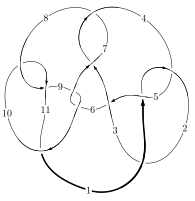
\includegraphics[width=112pt]{../../../GIT/diagram.site/Diagrams/png/621_11n_5.png}\\
\ \ \ A knot diagram\footnotemark}&
\allowdisplaybreaks
\textbf{Linearized knot diagam} \\
\cline{2-2}
 &
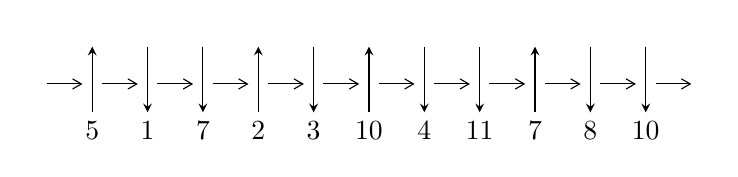
\begin{tikzpicture}[x=20pt, y=17pt]
	% nodes
	\node (C0) at (0, 0) {};
	\node (C1) at (1, 0) {};
	\node (C1U) at (1, +1) {};
	\node (C1D) at (1, -1) {5};

	\node (C2) at (2, 0) {};
	\node (C2U) at (2, +1) {};
	\node (C2D) at (2, -1) {1};

	\node (C3) at (3, 0) {};
	\node (C3U) at (3, +1) {};
	\node (C3D) at (3, -1) {7};

	\node (C4) at (4, 0) {};
	\node (C4U) at (4, +1) {};
	\node (C4D) at (4, -1) {2};

	\node (C5) at (5, 0) {};
	\node (C5U) at (5, +1) {};
	\node (C5D) at (5, -1) {3};

	\node (C6) at (6, 0) {};
	\node (C6U) at (6, +1) {};
	\node (C6D) at (6, -1) {10};

	\node (C7) at (7, 0) {};
	\node (C7U) at (7, +1) {};
	\node (C7D) at (7, -1) {4};

	\node (C8) at (8, 0) {};
	\node (C8U) at (8, +1) {};
	\node (C8D) at (8, -1) {11};

	\node (C9) at (9, 0) {};
	\node (C9U) at (9, +1) {};
	\node (C9D) at (9, -1) {7};

	\node (C10) at (10, 0) {};
	\node (C10U) at (10, +1) {};
	\node (C10D) at (10, -1) {8};

	\node (C11) at (11, 0) {};
	\node (C11U) at (11, +1) {};
	\node (C11D) at (11, -1) {10};
	\node (C12) at (12, 0) {};

	% arrows
	\draw[->,>={angle 60}]
	(C0) edge (C1) (C1) edge (C2) (C2) edge (C3) (C3) edge (C4) (C4) edge (C5) (C5) edge (C6) (C6) edge (C7) (C7) edge (C8) (C8) edge (C9) (C9) edge (C10) (C10) edge (C11) (C11) edge (C12) ;	\draw[->,>=stealth]
	(C1D) edge (C1U) (C2U) edge (C2D) (C3U) edge (C3D) (C4D) edge (C4U) (C5U) edge (C5D) (C6D) edge (C6U) (C7U) edge (C7D) (C8U) edge (C8D) (C9D) edge (C9U) (C10U) edge (C10D) (C11U) edge (C11D) ;
	\end{tikzpicture} \\
\hhline{~~} \\& 
\textbf{Solving Sequence} \\ \cline{2-2} 
 &
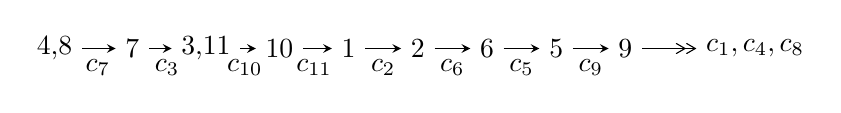
\begin{tikzpicture}[x=25pt, y=7pt]
	% node
	\node (A0) at (-1/8, 0) {4,8};
	\node (A1) at (1, 0) {7};
	\node (A2) at (33/16, 0) {3,11};
	\node (A3) at (25/8, 0) {10};
	\node (A4) at (33/8, 0) {1};
	\node (A5) at (41/8, 0) {2};
	\node (A6) at (49/8, 0) {6};
	\node (A7) at (57/8, 0) {5};
	\node (A8) at (65/8, 0) {9};
	\node (C1) at (1/2, -1) {$c_{7}$};
	\node (C2) at (3/2, -1) {$c_{3}$};
	\node (C3) at (21/8, -1) {$c_{10}$};
	\node (C4) at (29/8, -1) {$c_{11}$};
	\node (C5) at (37/8, -1) {$c_{2}$};
	\node (C6) at (45/8, -1) {$c_{6}$};
	\node (C7) at (53/8, -1) {$c_{5}$};
	\node (C8) at (61/8, -1) {$c_{9}$};
	\node (A9) at (10, 0) {$c_{1},c_{4},c_{8}$};

	% edge
	\draw[->,>=stealth]	
	(A0) edge (A1) (A1) edge (A2) (A2) edge (A3) (A3) edge (A4) (A4) edge (A5) (A5) edge (A6) (A6) edge (A7) (A7) edge (A8) ;
	\draw[->>,>={angle 60}]	
	(A8) edge (A9);
\end{tikzpicture} \\ 

\end{tabular} \\

\footnotetext{
The image of knot diagram is generated by the software ``\textbf{Draw programme}" developed by Andrew Bartholomew(\url{http://www.layer8.co.uk/maths/draw/index.htm\#Running-draw}), where we modified some parts for our purpose(\url{https://github.com/CATsTAILs/LinksPainter}).
}\phantom \\ \newline 
\centering \textbf{Ideals for irreducible components\footnotemark of $X_{\text{par}}$} 
 
\begin{align*}
I^u_{1}&=\langle 
2.93438\times10^{39} u^{39}+3.89993\times10^{39} u^{38}+\cdots+9.67095\times10^{39} b-1.11354\times10^{40},\\
\phantom{I^u_{1}}&\phantom{= \langle  }-5.08844\times10^{39} u^{39}+9.58525\times10^{38} u^{38}+\cdots+9.67095\times10^{39} a-1.38422\times10^{40},\;u^{40}+2 u^{39}+\cdots- u-1\rangle \\
I^u_{2}&=\langle 
b-1,\;u^4-2 u^3- u^2+a+3 u+1,\;u^5- u^4-2 u^3+u^2+u+1\rangle \\
\\
\end{align*}
\raggedright * 2 irreducible components of $\dim_{\mathbb{C}}=0$, with total 45 representations.\\
\footnotetext{All coefficients of polynomials are rational numbers. But the coefficients are sometimes approximated in decimal forms when there is not enough margin.}
\newpage
\renewcommand{\arraystretch}{1}
\centering \section*{I. $I^u_{1}= \langle 2.93\times10^{39} u^{39}+3.90\times10^{39} u^{38}+\cdots+9.67\times10^{39} b-1.11\times10^{40},\;-5.09\times10^{39} u^{39}+9.59\times10^{38} u^{38}+\cdots+9.67\times10^{39} a-1.38\times10^{40},\;u^{40}+2 u^{39}+\cdots- u-1 \rangle$}
\flushleft \textbf{(i) Arc colorings}\\
\begin{tabular}{m{7pt} m{180pt} m{7pt} m{180pt} }
\flushright $a_{4}=$&$\begin{pmatrix}0\\u\end{pmatrix}$ \\
\flushright $a_{8}=$&$\begin{pmatrix}1\\0\end{pmatrix}$ \\
\flushright $a_{7}=$&$\begin{pmatrix}1\\- u^2\end{pmatrix}$ \\
\flushright $a_{3}=$&$\begin{pmatrix}u\\- u^3+u\end{pmatrix}$ \\
\flushright $a_{11}=$&$\begin{pmatrix}0.526157 u^{39}-0.0991139 u^{38}+\cdots+1.57286 u+1.43132\\-0.303422 u^{39}-0.403263 u^{38}+\cdots+0.625271 u+1.15143\end{pmatrix}$ \\
\flushright $a_{10}=$&$\begin{pmatrix}0.222735 u^{39}-0.502377 u^{38}+\cdots+2.19813 u+2.58275\\-0.303422 u^{39}-0.403263 u^{38}+\cdots+0.625271 u+1.15143\end{pmatrix}$ \\
\flushright $a_{1}=$&$\begin{pmatrix}0.290241 u^{39}+0.200008 u^{38}+\cdots-1.21785 u-0.612287\\-0.120227 u^{39}-0.159505 u^{38}+\cdots+0.237926 u+0.0802655\end{pmatrix}$ \\
\flushright $a_{2}=$&$\begin{pmatrix}-0.578068 u^{39}-1.17622 u^{38}+\cdots+2.15345 u+1.24641\\-0.0185294 u^{39}-0.0980063 u^{38}+\cdots+1.25512 u-0.0172308\end{pmatrix}$ \\
\flushright $a_{6}=$&$\begin{pmatrix}0.410467 u^{39}+0.359513 u^{38}+\cdots-1.45577 u-0.692552\\-0.101647 u^{39}-0.257991 u^{38}+\cdots-0.186972 u+0.381156\end{pmatrix}$ \\
\flushright $a_{5}=$&$\begin{pmatrix}0.218303 u^{39}+0.00140845 u^{38}+\cdots-1.36554 u-0.312079\\-0.337234 u^{39}-0.662090 u^{38}+\cdots+0.0692011 u+0.735406\end{pmatrix}$ \\
\flushright $a_{9}=$&$\begin{pmatrix}0.278749 u^{39}-0.364781 u^{38}+\cdots+2.29798 u+2.37917\\-0.264706 u^{39}-0.351837 u^{38}+\cdots+0.543689 u+1.12586\end{pmatrix}$\\ \flushright $a_{9}=$&$\begin{pmatrix}0.278749 u^{39}-0.364781 u^{38}+\cdots+2.29798 u+2.37917\\-0.264706 u^{39}-0.351837 u^{38}+\cdots+0.543689 u+1.12586\end{pmatrix}$\\&\end{tabular}
\flushleft \textbf{(ii) Obstruction class $= -1$}\\~\\
\flushleft \textbf{(iii) Cusp Shapes $= 0.625380 u^{39}-2.23284 u^{38}+\cdots+22.1362 u-1.81055$}\\~\\
\newpage\renewcommand{\arraystretch}{1}
\flushleft \textbf{(iv) u-Polynomials at the component}\newline \\
\begin{tabular}{m{50pt}|m{274pt}}
Crossings & \hspace{64pt}u-Polynomials at each crossing \\
\hline $$\begin{aligned}c_{1},c_{4}\end{aligned}$$&$\begin{aligned}
&u^{40}+2 u^{39}+\cdots+5 u+1
\end{aligned}$\\
\hline $$\begin{aligned}c_{2}\end{aligned}$$&$\begin{aligned}
&u^{40}+18 u^{39}+\cdots- u+1
\end{aligned}$\\
\hline $$\begin{aligned}c_{3},c_{7}\end{aligned}$$&$\begin{aligned}
&u^{40}+2 u^{39}+\cdots- u-1
\end{aligned}$\\
\hline $$\begin{aligned}c_{5}\end{aligned}$$&$\begin{aligned}
&u^{40}-2 u^{39}+\cdots+61 u+17
\end{aligned}$\\
\hline $$\begin{aligned}c_{6},c_{9}\end{aligned}$$&$\begin{aligned}
&u^{40}+5 u^{39}+\cdots+64 u+32
\end{aligned}$\\
\hline $$\begin{aligned}c_{8},c_{10}\end{aligned}$$&$\begin{aligned}
&u^{40}-6 u^{39}+\cdots-5 u-1
\end{aligned}$\\
\hline $$\begin{aligned}c_{11}\end{aligned}$$&$\begin{aligned}
&u^{40}+14 u^{39}+\cdots+23 u+1
\end{aligned}$\\
\hline
\end{tabular}\\~\\
\newpage\renewcommand{\arraystretch}{1}
\flushleft \textbf{(v) Riley Polynomials at the component}\newline \\
\begin{tabular}{m{50pt}|m{274pt}}
Crossings & \hspace{64pt}Riley Polynomials at each crossing \\
\hline $$\begin{aligned}c_{1},c_{4}\end{aligned}$$&$\begin{aligned}
&y^{40}+18 y^{39}+\cdots- y+1
\end{aligned}$\\
\hline $$\begin{aligned}c_{2}\end{aligned}$$&$\begin{aligned}
&y^{40}+10 y^{39}+\cdots-101 y+1
\end{aligned}$\\
\hline $$\begin{aligned}c_{3},c_{7}\end{aligned}$$&$\begin{aligned}
&y^{40}-10 y^{39}+\cdots- y+1
\end{aligned}$\\
\hline $$\begin{aligned}c_{5}\end{aligned}$$&$\begin{aligned}
&y^{40}+2 y^{39}+\cdots+223 y+289
\end{aligned}$\\
\hline $$\begin{aligned}c_{6},c_{9}\end{aligned}$$&$\begin{aligned}
&y^{40}-33 y^{39}+\cdots-8704 y+1024
\end{aligned}$\\
\hline $$\begin{aligned}c_{8},c_{10}\end{aligned}$$&$\begin{aligned}
&y^{40}-14 y^{39}+\cdots-23 y+1
\end{aligned}$\\
\hline $$\begin{aligned}c_{11}\end{aligned}$$&$\begin{aligned}
&y^{40}+30 y^{39}+\cdots+89 y+1
\end{aligned}$\\
\hline
\end{tabular}\\~\\
\newpage\flushleft \textbf{(vi) Complex Volumes and Cusp Shapes}
$$\begin{array}{c|c|c}  
\text{Solutions to }I^u_{1}& \I (\text{vol} + \sqrt{-1}CS) & \text{Cusp shape}\\
 \hline 
\begin{aligned}
u &= \phantom{-}0.752901 + 0.442189 I \\
a &= -0.604966 + 0.350008 I \\
b &= \phantom{-}0.829023 + 0.938697 I\end{aligned}
 & -1.98806 - 6.13047 I & -7.04352 + 9.47962 I \\ \hline\begin{aligned}
u &= \phantom{-}0.752901 - 0.442189 I \\
a &= -0.604966 - 0.350008 I \\
b &= \phantom{-}0.829023 - 0.938697 I\end{aligned}
 & -1.98806 + 6.13047 I & -7.04352 - 9.47962 I \\ \hline\begin{aligned}
u &= -0.655458 + 0.476008 I \\
a &= -0.318936 - 0.554304 I \\
b &= \phantom{-}0.613689 - 0.710479 I\end{aligned}
 & -0.42554 + 1.82346 I & -2.95478 - 4.65601 I \\ \hline\begin{aligned}
u &= -0.655458 - 0.476008 I \\
a &= -0.318936 + 0.554304 I \\
b &= \phantom{-}0.613689 + 0.710479 I\end{aligned}
 & -0.42554 - 1.82346 I & -2.95478 + 4.65601 I \\ \hline\begin{aligned}
u &= -0.810417 + 0.872688 I \\
a &= \phantom{-}0.140090 + 0.325947 I \\
b &= -0.551174 - 1.182170 I\end{aligned}
 & \phantom{-}4.57008 + 7.07850 I & -2.02910 - 5.97329 I \\ \hline\begin{aligned}
u &= -0.810417 - 0.872688 I \\
a &= \phantom{-}0.140090 - 0.325947 I \\
b &= -0.551174 + 1.182170 I\end{aligned}
 & \phantom{-}4.57008 - 7.07850 I & -2.02910 + 5.97329 I \\ \hline\begin{aligned}
u &= -0.643082 + 1.012100 I \\
a &= \phantom{-}0.398027 + 0.191743 I \\
b &= -0.617281 - 0.666490 I\end{aligned}
 & \phantom{-}0.145121 + 0.763133 I & -4.51767 - 0.23788 I \\ \hline\begin{aligned}
u &= -0.643082 - 1.012100 I \\
a &= \phantom{-}0.398027 - 0.191743 I \\
b &= -0.617281 + 0.666490 I\end{aligned}
 & \phantom{-}0.145121 - 0.763133 I & -4.51767 + 0.23788 I \\ \hline\begin{aligned}
u &= \phantom{-}0.799783 + 0.916888 I \\
a &= \phantom{-}0.215570 - 0.335982 I \\
b &= -0.650453 + 1.082920 I\end{aligned}
 & \phantom{-}6.09690 - 1.71389 I & \phantom{-}0.373315 + 0.701321 I \\ \hline\begin{aligned}
u &= \phantom{-}0.799783 - 0.916888 I \\
a &= \phantom{-}0.215570 + 0.335982 I \\
b &= -0.650453 - 1.082920 I\end{aligned}
 & \phantom{-}6.09690 + 1.71389 I & \phantom{-}0.373315 - 0.701321 I\\
 \hline 
 \end{array}$$\newpage$$\begin{array}{c|c|c}  
\text{Solutions to }I^u_{1}& \I (\text{vol} + \sqrt{-1}CS) & \text{Cusp shape}\\
 \hline 
\begin{aligned}
u &= \phantom{-}0.711514 + 0.271124 I \\
a &= -1.148250 + 0.635421 I \\
b &= \phantom{-}1.174800 + 0.553857 I\end{aligned}
 & -3.56782 - 0.26795 I & -11.60981 + 1.69985 I \\ \hline\begin{aligned}
u &= \phantom{-}0.711514 - 0.271124 I \\
a &= -1.148250 - 0.635421 I \\
b &= \phantom{-}1.174800 - 0.553857 I\end{aligned}
 & -3.56782 + 0.26795 I & -11.60981 - 1.69985 I \\ \hline\begin{aligned}
u &= -0.753278 + 0.081360 I \\
a &= -1.63901 - 0.21826 I \\
b &= \phantom{-}1.50673 - 0.20107 I\end{aligned}
 & -4.40562 + 3.00647 I & -12.14909 - 4.76014 I \\ \hline\begin{aligned}
u &= -0.753278 - 0.081360 I \\
a &= -1.63901 + 0.21826 I \\
b &= \phantom{-}1.50673 + 0.20107 I\end{aligned}
 & -4.40562 - 3.00647 I & -12.14909 + 4.76014 I \\ \hline\begin{aligned}
u &= -1.028320 + 0.763633 I \\
a &= \phantom{-}1.61875 + 0.32346 I \\
b &= -0.801483 + 0.818338 I\end{aligned}
 & \phantom{-}3.86288 - 0.92225 I & -2.44177 - 0.36369 I \\ \hline\begin{aligned}
u &= -1.028320 - 0.763633 I \\
a &= \phantom{-}1.61875 - 0.32346 I \\
b &= -0.801483 - 0.818338 I\end{aligned}
 & \phantom{-}3.86288 + 0.92225 I & -2.44177 + 0.36369 I \\ \hline\begin{aligned}
u &= \phantom{-}0.797251 + 1.038720 I \\
a &= \phantom{-}0.390573 - 0.367350 I \\
b &= -0.878605 + 0.846502 I\end{aligned}
 & \phantom{-}5.41673 + 1.52162 I & \phantom{-0.000000 }      -6
0. 10   - 0.682803 I \\ \hline\begin{aligned}
u &= \phantom{-}0.797251 - 1.038720 I \\
a &= \phantom{-}0.390573 + 0.367350 I \\
b &= -0.878605 - 0.846502 I\end{aligned}
 & \phantom{-}5.41673 - 1.52162 I & \phantom{-0.000000 -}     -6
0. 10   + 0.682803 I \\ \hline\begin{aligned}
u &= -0.422420 + 0.531130 I \\
a &= \phantom{-}0.580600 - 0.488478 I \\
b &= \phantom{-}0.175715 - 0.238829 I\end{aligned}
 & -0.196422 + 1.363410 I & -2.16894 - 4.86353 I \\ \hline\begin{aligned}
u &= -0.422420 - 0.531130 I \\
a &= \phantom{-}0.580600 + 0.488478 I \\
b &= \phantom{-}0.175715 + 0.238829 I\end{aligned}
 & -0.196422 - 1.363410 I & -2.16894 + 4.86353 I\\
 \hline 
 \end{array}$$\newpage$$\begin{array}{c|c|c}  
\text{Solutions to }I^u_{1}& \I (\text{vol} + \sqrt{-1}CS) & \text{Cusp shape}\\
 \hline 
\begin{aligned}
u &= \phantom{-}1.054050 + 0.808417 I \\
a &= \phantom{-}1.58951 - 0.38241 I \\
b &= -0.921400 - 0.829719 I\end{aligned}
 & \phantom{-}5.28266 - 4.71026 I & \phantom{-0.000000 -}0. + 5.00895 I \\ \hline\begin{aligned}
u &= \phantom{-}1.054050 - 0.808417 I \\
a &= \phantom{-}1.58951 + 0.38241 I \\
b &= -0.921400 + 0.829719 I\end{aligned}
 & \phantom{-}5.28266 + 4.71026 I & \phantom{-0.000000 } 0. - 5.00895 I \\ \hline\begin{aligned}
u &= -1.35764\phantom{ +0.000000I} \\
a &= \phantom{-}1.36371\phantom{ +0.000000I} \\
b &= -0.670384\phantom{ +0.000000I}\end{aligned}
 & -3.32615\phantom{ +0.000000I} & \phantom{-}1.98010\phantom{ +0.000000I} \\ \hline\begin{aligned}
u &= -0.816149 + 1.085630 I \\
a &= \phantom{-}0.451733 + 0.389885 I \\
b &= -0.971878 - 0.771756 I\end{aligned}
 & \phantom{-}3.33510 - 6.89323 I & -3.00000 + 5.25790 I \\ \hline\begin{aligned}
u &= -0.816149 - 1.085630 I \\
a &= \phantom{-}0.451733 - 0.389885 I \\
b &= -0.971878 + 0.771756 I\end{aligned}
 & \phantom{-}3.33510 + 6.89323 I & -3.00000 - 5.25790 I \\ \hline\begin{aligned}
u &= -0.460095 + 0.445935 I \\
a &= \phantom{-}1.143080 - 0.772133 I \\
b &= \phantom{-}0.315005 + 0.068617 I\end{aligned}
 & -0.154276 + 1.379410 I & -2.57505 - 4.68653 I \\ \hline\begin{aligned}
u &= -0.460095 - 0.445935 I \\
a &= \phantom{-}1.143080 + 0.772133 I \\
b &= \phantom{-}0.315005 - 0.068617 I\end{aligned}
 & -0.154276 - 1.379410 I & -2.57505 + 4.68653 I \\ \hline\begin{aligned}
u &= \phantom{-}0.392808 + 0.498293 I \\
a &= \phantom{-}1.96044 + 1.55878 I \\
b &= \phantom{-}0.700490 - 0.229460 I\end{aligned}
 & -1.02172 + 2.83866 I & -5.26921 + 0.34131 I \\ \hline\begin{aligned}
u &= \phantom{-}0.392808 - 0.498293 I \\
a &= \phantom{-}1.96044 - 1.55878 I \\
b &= \phantom{-}0.700490 + 0.229460 I\end{aligned}
 & -1.02172 - 2.83866 I & -5.26921 - 0.34131 I \\ \hline\begin{aligned}
u &= \phantom{-}1.093020 + 0.888850 I \\
a &= \phantom{-}1.51810 - 0.48663 I \\
b &= -1.155200 - 0.809789 I\end{aligned}
 & \phantom{-}4.47319 - 8.54344 I & \phantom{-0.000000 -}0. + 4.74667 I\\
 \hline 
 \end{array}$$\newpage$$\begin{array}{c|c|c}  
\text{Solutions to }I^u_{1}& \I (\text{vol} + \sqrt{-1}CS) & \text{Cusp shape}\\
 \hline 
\begin{aligned}
u &= \phantom{-}1.093020 - 0.888850 I \\
a &= \phantom{-}1.51810 + 0.48663 I \\
b &= -1.155200 + 0.809789 I\end{aligned}
 & \phantom{-}4.47319 + 8.54344 I & \phantom{-0.000000 } 0. - 4.74667 I \\ \hline\begin{aligned}
u &= \phantom{-}0.577742\phantom{ +0.000000I} \\
a &= -2.60696\phantom{ +0.000000I} \\
b &= \phantom{-}1.20395\phantom{ +0.000000I}\end{aligned}
 & -2.39024\phantom{ +0.000000I} & -2.93570\phantom{ +0.000000I} \\ \hline\begin{aligned}
u &= -1.14394 + 0.85054 I \\
a &= \phantom{-}1.46853 + 0.41523 I \\
b &= -1.082180 + 0.668751 I\end{aligned}
 & -1.33633 + 6.06144 I & \phantom{-0.000000 } 0 \\ \hline\begin{aligned}
u &= -1.14394 - 0.85054 I \\
a &= \phantom{-}1.46853 - 0.41523 I \\
b &= -1.082180 - 0.668751 I\end{aligned}
 & -1.33633 - 6.06144 I & \phantom{-0.000000 } 0 \\ \hline\begin{aligned}
u &= -1.10053 + 0.91184 I \\
a &= \phantom{-}1.49517 + 0.51717 I \\
b &= -1.22599 + 0.79743 I\end{aligned}
 & \phantom{-}2.4064 + 14.1156 I & \phantom{-0.000000 } 0. - 8.71801 I \\ \hline\begin{aligned}
u &= -1.10053 - 0.91184 I \\
a &= \phantom{-}1.49517 - 0.51717 I \\
b &= -1.22599 - 0.79743 I\end{aligned}
 & \phantom{-}2.4064 - 14.1156 I & \phantom{-0.000000 -}0. + 8.71801 I \\ \hline\begin{aligned}
u &= \phantom{-}1.51868 + 0.20012 I \\
a &= \phantom{-}1.325660 - 0.048656 I \\
b &= -0.767634 - 0.087671 I\end{aligned}
 & -7.01606 - 4.59273 I & \phantom{-0.000000 } 0 \\ \hline\begin{aligned}
u &= \phantom{-}1.51868 - 0.20012 I \\
a &= \phantom{-}1.325660 + 0.048656 I \\
b &= -0.767634 + 0.087671 I\end{aligned}
 & -7.01606 + 4.59273 I & \phantom{-0.000000 } 0 \\ \hline\begin{aligned}
u &= \phantom{-}0.103618 + 0.421336 I \\
a &= \phantom{-}6.03694 + 2.30128 I \\
b &= \phantom{-}1.041040 - 0.055984 I\end{aligned}
 & -1.92691 - 1.82552 I & \phantom{-}15.7454 + 26.9436 I \\ \hline\begin{aligned}
u &= \phantom{-}0.103618 - 0.421336 I \\
a &= \phantom{-}6.03694 - 2.30128 I \\
b &= \phantom{-}1.041040 + 0.055984 I\end{aligned}
 & -1.92691 + 1.82552 I & \phantom{-}15.7454 - 26.9436 I\\
 \hline 
 \end{array}$$\newpage\newpage\renewcommand{\arraystretch}{1}
\centering \section*{II. $I^u_{2}= \langle b-1,\;u^4-2 u^3- u^2+a+3 u+1,\;u^5- u^4-2 u^3+u^2+u+1 \rangle$}
\flushleft \textbf{(i) Arc colorings}\\
\begin{tabular}{m{7pt} m{180pt} m{7pt} m{180pt} }
\flushright $a_{4}=$&$\begin{pmatrix}0\\u\end{pmatrix}$ \\
\flushright $a_{8}=$&$\begin{pmatrix}1\\0\end{pmatrix}$ \\
\flushright $a_{7}=$&$\begin{pmatrix}1\\- u^2\end{pmatrix}$ \\
\flushright $a_{3}=$&$\begin{pmatrix}u\\- u^3+u\end{pmatrix}$ \\
\flushright $a_{11}=$&$\begin{pmatrix}- u^4+2 u^3+u^2-3 u-1\\1\end{pmatrix}$ \\
\flushright $a_{10}=$&$\begin{pmatrix}- u^4+2 u^3+u^2-3 u\\1\end{pmatrix}$ \\
\flushright $a_{1}=$&$\begin{pmatrix}-1\\0\end{pmatrix}$ \\
\flushright $a_{2}=$&$\begin{pmatrix}- u^3+2 u\\- u^3+u\end{pmatrix}$ \\
\flushright $a_{6}=$&$\begin{pmatrix}1\\- u^2\end{pmatrix}$ \\
\flushright $a_{5}=$&$\begin{pmatrix}- u^2+1\\u^4-2 u^2\end{pmatrix}$ \\
\flushright $a_{9}=$&$\begin{pmatrix}- u^4+2 u^3+u^2-3 u\\1\end{pmatrix}$\\ \flushright $a_{9}=$&$\begin{pmatrix}- u^4+2 u^3+u^2-3 u\\1\end{pmatrix}$\\&\end{tabular}
\flushleft \textbf{(ii) Obstruction class $= 1$}\\~\\
\flushleft \textbf{(iii) Cusp Shapes $= 2 u^4+u^3-7 u^2-3 u-6$}\\~\\
\newpage\renewcommand{\arraystretch}{1}
\flushleft \textbf{(iv) u-Polynomials at the component}\newline \\
\begin{tabular}{m{50pt}|m{274pt}}
Crossings & \hspace{64pt}u-Polynomials at each crossing \\
\hline $$\begin{aligned}c_{1}\end{aligned}$$&$\begin{aligned}
&u^5- u^4+2 u^3- u^2+u-1
\end{aligned}$\\
\hline $$\begin{aligned}c_{2}\end{aligned}$$&$\begin{aligned}
&u^5+3 u^4+4 u^3+u^2- u-1
\end{aligned}$\\
\hline $$\begin{aligned}c_{3}\end{aligned}$$&$\begin{aligned}
&u^5+u^4-2 u^3- u^2+u-1
\end{aligned}$\\
\hline $$\begin{aligned}c_{4}\end{aligned}$$&$\begin{aligned}
&u^5+u^4+2 u^3+u^2+u+1
\end{aligned}$\\
\hline $$\begin{aligned}c_{5},c_{7}\end{aligned}$$&$\begin{aligned}
&u^5- u^4-2 u^3+u^2+u+1
\end{aligned}$\\
\hline $$\begin{aligned}c_{6},c_{9}\end{aligned}$$&$\begin{aligned}
&u^5
\end{aligned}$\\
\hline $$\begin{aligned}c_{8}\end{aligned}$$&$\begin{aligned}
&(u-1)^5
\end{aligned}$\\
\hline $$\begin{aligned}c_{10},c_{11}\end{aligned}$$&$\begin{aligned}
&(u+1)^5
\end{aligned}$\\
\hline
\end{tabular}\\~\\
\newpage\renewcommand{\arraystretch}{1}
\flushleft \textbf{(v) Riley Polynomials at the component}\newline \\
\begin{tabular}{m{50pt}|m{274pt}}
Crossings & \hspace{64pt}Riley Polynomials at each crossing \\
\hline $$\begin{aligned}c_{1},c_{4}\end{aligned}$$&$\begin{aligned}
&y^5+3 y^4+4 y^3+y^2- y-1
\end{aligned}$\\
\hline $$\begin{aligned}c_{2}\end{aligned}$$&$\begin{aligned}
&y^5- y^4+8 y^3-3 y^2+3 y-1
\end{aligned}$\\
\hline $$\begin{aligned}c_{3},c_{5},c_{7}\end{aligned}$$&$\begin{aligned}
&y^5-5 y^4+8 y^3-3 y^2- y-1
\end{aligned}$\\
\hline $$\begin{aligned}c_{6},c_{9}\end{aligned}$$&$\begin{aligned}
&y^5
\end{aligned}$\\
\hline $$\begin{aligned}c_{8},c_{10},c_{11}\end{aligned}$$&$\begin{aligned}
&(y-1)^5
\end{aligned}$\\
\hline
\end{tabular}\\~\\
\newpage\flushleft \textbf{(vi) Complex Volumes and Cusp Shapes}
$$\begin{array}{c|c|c}  
\text{Solutions to }I^u_{2}& \I (\text{vol} + \sqrt{-1}CS) & \text{Cusp shape}\\
 \hline 
\begin{aligned}
u &= -1.21774\phantom{ +0.000000I} \\
a &= -1.67436\phantom{ +0.000000I} \\
b &= \phantom{-}1.00000\phantom{ +0.000000I}\end{aligned}
 & -4.04602\phantom{ +0.000000I} & -10.1350\phantom{ +0.000000I} \\ \hline\begin{aligned}
u &= -0.309916 + 0.549911 I \\
a &= \phantom{-}0.29977 - 2.14694 I \\
b &= \phantom{-}1.00000\phantom{ +0.000000I}\end{aligned}
 & -1.97403 + 1.53058 I & -3.52158 + 1.00973 I \\ \hline\begin{aligned}
u &= -0.309916 - 0.549911 I \\
a &= \phantom{-}0.29977 + 2.14694 I \\
b &= \phantom{-}1.00000\phantom{ +0.000000I}\end{aligned}
 & -1.97403 - 1.53058 I & -3.52158 - 1.00973 I \\ \hline\begin{aligned}
u &= \phantom{-}1.41878 + 0.21917 I \\
a &= -1.46259 + 0.14641 I \\
b &= \phantom{-}1.00000\phantom{ +0.000000I}\end{aligned}
 & -7.51750 - 4.40083 I & -14.4110 + 1.1901 I \\ \hline\begin{aligned}
u &= \phantom{-}1.41878 - 0.21917 I \\
a &= -1.46259 - 0.14641 I \\
b &= \phantom{-}1.00000\phantom{ +0.000000I}\end{aligned}
 & -7.51750 + 4.40083 I & -14.4110 - 1.1901 I\\
 \hline 
 \end{array}$$\newpage
\newpage\renewcommand{\arraystretch}{1}
\centering \section*{ III. u-Polynomials}
\begin{tabular}{m{50pt}|m{274pt}}
Crossings & \hspace{64pt}u-Polynomials at each crossing \\
\hline $$\begin{aligned}c_{1}\end{aligned}$$&$\begin{aligned}
&(u^5- u^4+2 u^3- u^2+u-1)(u^{40}+2 u^{39}+\cdots+5 u+1)
\end{aligned}$\\
\hline $$\begin{aligned}c_{2}\end{aligned}$$&$\begin{aligned}
&(u^5+3 u^4+4 u^3+u^2- u-1)(u^{40}+18 u^{39}+\cdots- u+1)
\end{aligned}$\\
\hline $$\begin{aligned}c_{3}\end{aligned}$$&$\begin{aligned}
&(u^5+u^4-2 u^3- u^2+u-1)(u^{40}+2 u^{39}+\cdots- u-1)
\end{aligned}$\\
\hline $$\begin{aligned}c_{4}\end{aligned}$$&$\begin{aligned}
&(u^5+u^4+2 u^3+u^2+u+1)(u^{40}+2 u^{39}+\cdots+5 u+1)
\end{aligned}$\\
\hline $$\begin{aligned}c_{5}\end{aligned}$$&$\begin{aligned}
&(u^5- u^4-2 u^3+u^2+u+1)(u^{40}-2 u^{39}+\cdots+61 u+17)
\end{aligned}$\\
\hline $$\begin{aligned}c_{6},c_{9}\end{aligned}$$&$\begin{aligned}
&u^5(u^{40}+5 u^{39}+\cdots+64 u+32)
\end{aligned}$\\
\hline $$\begin{aligned}c_{7}\end{aligned}$$&$\begin{aligned}
&(u^5- u^4-2 u^3+u^2+u+1)(u^{40}+2 u^{39}+\cdots- u-1)
\end{aligned}$\\
\hline $$\begin{aligned}c_{8}\end{aligned}$$&$\begin{aligned}
&((u-1)^5)(u^{40}-6 u^{39}+\cdots-5 u-1)
\end{aligned}$\\
\hline $$\begin{aligned}c_{10}\end{aligned}$$&$\begin{aligned}
&((u+1)^5)(u^{40}-6 u^{39}+\cdots-5 u-1)
\end{aligned}$\\
\hline $$\begin{aligned}c_{11}\end{aligned}$$&$\begin{aligned}
&((u+1)^5)(u^{40}+14 u^{39}+\cdots+23 u+1)
\end{aligned}$\\
\hline
\end{tabular}\newpage\renewcommand{\arraystretch}{1}
\centering \section*{ IV. Riley Polynomials}
\begin{tabular}{m{50pt}|m{274pt}}
Crossings & \hspace{64pt}Riley Polynomials at each crossing \\
\hline $$\begin{aligned}c_{1},c_{4}\end{aligned}$$&$\begin{aligned}
&(y^5+3 y^4+4 y^3+y^2- y-1)(y^{40}+18 y^{39}+\cdots- y+1)
\end{aligned}$\\
\hline $$\begin{aligned}c_{2}\end{aligned}$$&$\begin{aligned}
&(y^5- y^4+8 y^3-3 y^2+3 y-1)(y^{40}+10 y^{39}+\cdots-101 y+1)
\end{aligned}$\\
\hline $$\begin{aligned}c_{3},c_{7}\end{aligned}$$&$\begin{aligned}
&(y^5-5 y^4+8 y^3-3 y^2- y-1)(y^{40}-10 y^{39}+\cdots- y+1)
\end{aligned}$\\
\hline $$\begin{aligned}c_{5}\end{aligned}$$&$\begin{aligned}
&(y^5-5 y^4+8 y^3-3 y^2- y-1)(y^{40}+2 y^{39}+\cdots+223 y+289)
\end{aligned}$\\
\hline $$\begin{aligned}c_{6},c_{9}\end{aligned}$$&$\begin{aligned}
&y^5(y^{40}-33 y^{39}+\cdots-8704 y+1024)
\end{aligned}$\\
\hline $$\begin{aligned}c_{8},c_{10}\end{aligned}$$&$\begin{aligned}
&((y-1)^5)(y^{40}-14 y^{39}+\cdots-23 y+1)
\end{aligned}$\\
\hline $$\begin{aligned}c_{11}\end{aligned}$$&$\begin{aligned}
&((y-1)^5)(y^{40}+30 y^{39}+\cdots+89 y+1)
\end{aligned}$\\
\hline
\end{tabular}
\vskip 2pc
\end{document}